\documentclass[../main.tex]{subfiles}
\graphicspath{{\subfix{../images/}}} % Images path

\begin{document}

\section{Dataset Description}\label{sec:dataset-description}

The dataset adopted for the implementation and the assessment of the BoW classifier in this study is the \textit{15-Scenes} dataset from \textit{Lazebnik et al.} [TODO:reference]. This dataset consists of a total of $4485$ grayscale images, each belonging to one of $15$ different scene categories (\itt{office, kitchen, living room, bedroom, store, industrial, tall building, inside city, street, highway, coast, open country, mountain, forest, suburb}). The images come already splitted into a training set of $1500$ images, with a uniform distribution of $100$ images per category, and a test set of $2985$ images, for which the distribution of images is not uniform as shown in Figure~\ref{fig:dataset-distribution}.

\begin{figure}[H]
  \centering
  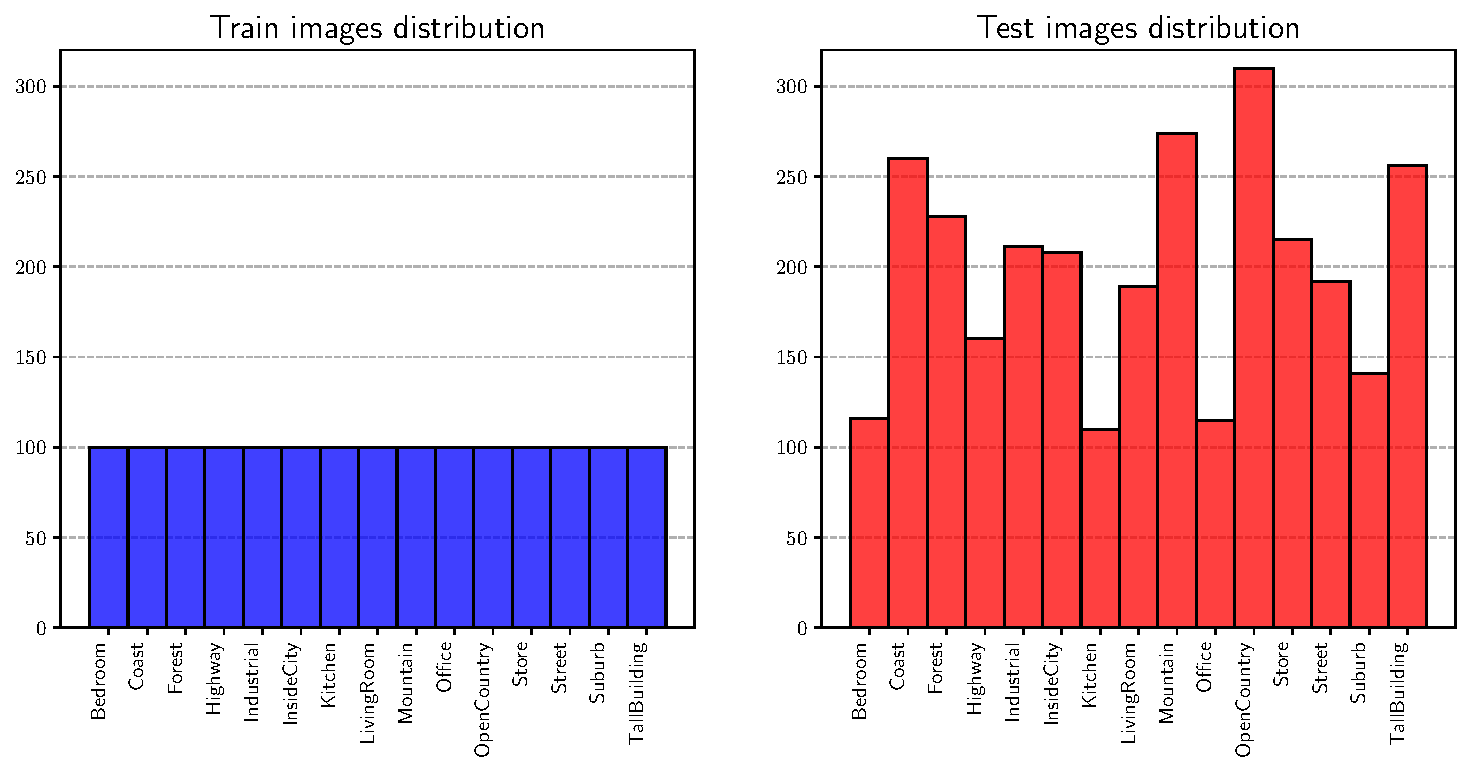
\includegraphics[width=\textwidth]{classes_distribution.pdf}
  \caption{Distribution of images in train and test sets for the \itt{15-Scenes} dataset.}
  \label{fig:dataset-distribution}
\end{figure}

%  Therefore, it's already possible to mention that the accuracy of the dummy classifier (that always predicts the most frequent class) on the test set is $10.39\%$, and will be used as baseline for comparison of the next classifiers.\\
Moreover, it's worth mentioning that the images in the dataset are of different sizes and aspect ratios, with the vaste majority of them being $256 \times 256$ pixels. This is an important aspect to consider since it directly impacts the feature extraction phase as explained in Section~\ref{sec:visual-vocabulary-construction}.

\end{document}

